\section{Theoretische Grundlagen}
    \subsection{Allgemeines}
        Schallwellen sind longitudinale Schwingungen von Teilchen in einem Medium und sie können mithilfe der sogenannten Helmholtzgleichung mathematisch beschrieben werden:
        \begin{equation*}
            \Delta P(\vec{r},t) = \frac{1}{c^2} \frac{\partial^2 P(\vec{r},t)}{\partial t^2}
        \end{equation*}
        $P(\vec{r},t)$ beschreibt hierbei die Verteilung der Druckamplitude und $c$ ist die Ausbreitungsgeschindigkeit/Gruppengeschwindgkeit der Welle.
        Nach dem Abseparieren der Zeitabhängigkeit nach $P(\vec{r},t) = p(\vec{r}) \cdot \cos(\omega t)$ ergibt sich eine stationäre Differentialgleichung für den Druck.
        \begin{equation}
            \Delta p(\vec{r}) = \frac{\omega^2}{c^2} p(\vec{r})
            \label{eqn:helmholtz}
        \end{equation}

        Analog wird die Wellenfunktion, deren Betragsquadrat die Wahrscheinlichkeitsdichte eines Elektrons ist, in einem zeitunabhängigen Potential $V(\vec{r})$ mithilfe der Schrödingergleichung
        \begin{equation*}
            -\frac{\hbar^2}{2m} \Delta \Psi(\vec{r},t) + V(\vec{r}) \Psi(\vec{r},t) = i\hbar \frac{\partial}{\partial t} \Psi(\vec{r},t)
        \end{equation*}
        bestimmt. Auch hier wird die Zeitabhängigkeit über $\Psi(\vec{r},t) = \psi(\vec{r}) \cdot e^{-i \omega t}$ abgekoppelt, was wiederum zur stationären Schrödingergleichung führt:
        \begin{equation}
            -\frac{\hbar^2}{2m} \Delta \psi(\vec{r}) + V(\vec{r}) \psi(\vec{r}) = E \psi(\vec{r})
            \label{eqn:schrödinger}
        \end{equation}

        Das Analogon zum Potential, in welchem sich das Elektron befindet, ist das Einschließen des Gases in einem Volumen $V$.
        Dabei gelten die Von-Neuman-Randbedingungen
        \begin{equation*}
            \vec{\nabla} P(\vec{r},t) |_{\partial V} = 0
        \end{equation*}
        an den Grenzen des Volumens. \\
        Die dabei unter unter konstruktiver Interferenz der einfallenden und der am Rand des Volumens reflektierten Welle entstehenden stehenden Wellen können als das Analogon zu Wellenfunktionen von bestimmten quantenmechanischen Systemen benutzt werden.

    \subsection{Unendlicher Potentialtopf}
        \subsubsection*{Potentialtopf}
            Der eindimensionale unendliche Potentialtopf mit dem Potential
            \begin{equation*}
                V(x) =
                \begin{cases}
                    0,      & 0\leq x \leq L \\
                    \infty, & \text{sonst}
                \end{cases}
            \end{equation*}
            wird mit der stationären Schrödingergleichung
            \begin{equation*}
                \frac{\partial^2}{\partial x^2} \psi(x) + V(x) \psi(x) = E \psi(x)
            \end{equation*}
            und den Randbedingungen
            \begin{equation*}
                \psi(0) = \psi(L) = 0
            \end{equation*}
            gelöst. Es ergibt sich eine ebene Welle,
            \begin{equation*}
                \psi(x) = A \sin(kx)
            \end{equation*}
            deren Extrema sich im Laufe der Zeit nicht verschieben (stehende Welle) mit der Kreiswellenzahl:
            \begin{equation}
                k = \frac{\pi n}{L} \qquad \text{mit} \qquad n \in \mathbb{N}
                \label{eqn:kPotentialtopf}
            \end{equation}

            \begin{figure}[h]
                \centering
                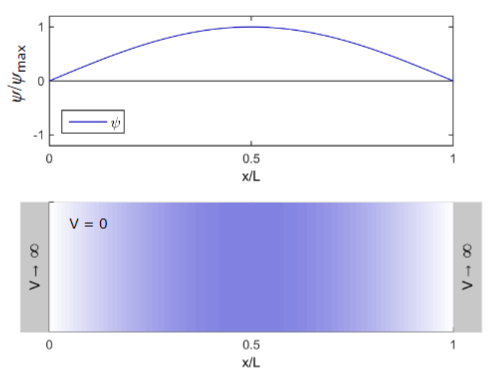
\includegraphics[scale=0.6]{pictures/Potentialtopf.png}
                \caption{Hier wird beispielhaft die Lösung der Schrödingergleichung für einen unendlichen Potentialtopf $\psi(x)$ mit $n=1$ dargestellt. Entnommen aus \cite{httpsapphysikuni-konstanzdeap-publicanleitungenquantenmodelle-teil1pdf_quantenmodelle-teil1pdf_nodate}.}
                \label{fig:Potentialtopf}
            \end{figure}

            \FloatBarrier

        \subsubsection*{Rohrresonator und Analogon}
            Hierbei wird an einem Ende eines Rohres ein Lautsprecher und am anderen Ende ein Mikrofon angebracht. Es wird von Resonanz gesprochen, wenn eine stehende Welle durch konstruktive Überlagerung der vom Lautsprecher einfallenden und der reflektierten Schallwelle ensteht. Dabei muss die Länge des Rohres ein ganzzahliges Vielfaches der halben Wellenlänge der Schallwelle sein:
            \begin{equation*}
                L = \frac{\lambda}{2} n
            \end{equation*}
            Mit der Definition der Kreiswellenzahl $k = \frac{2\pi}{\lambda}$ ergibt sich die gleiche Bedingung wie für den unendlichen Potentialtopf in \eqref{eqn:kPotentialtopf}:
            \begin{equation*}
                k = \frac{\pi n}{L} \qquad \text{mit} \qquad n \in \mathbb{N}
            \end{equation*}

            \begin{figure}[h]
                \centering
                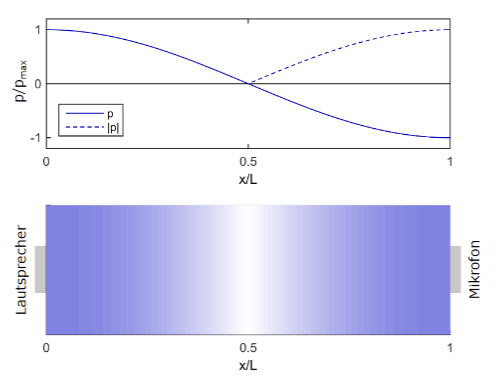
\includegraphics[scale=0.6]{pictures/Rohrresonator.png}
                \caption{Hier wird beispielhaft die Druckamplitude eines Rohrresonators $p(x)$ mit $n=1$ dargestellt. Entnommen aus \cite{httpsapphysikuni-konstanzdeap-publicanleitungenquantenmodelle-teil1pdf_quantenmodelle-teil1pdf_nodate}.}
                \label{fig:Rohrresonator}
            \end{figure}

            \FloatBarrier

            Der einzige Unterschied zwischen der Druckverteilung $p(x)$ und der Wellenfunktion $\psi(x)$ liegt in der Position der Knoten und Bäuche, aufgrund der verschiedenen Randbedingungen, wie es in \autoref{fig:Potentialtopf} und \autoref{fig:Rohrresonator} zu erkennen ist.
            
    \subsection{Wasserstoffatom und Analogon}
        \subsubsection*{Wasserstoffatom}
            Die Wellenfunktion für das Wasserstoffatom wird auch mit der stationären Schrödingergleichung \eqref{eqn:schrödinger} bestimmt. Wegen der Kugelsymmetrie des Coulombpotentials des Kerns $V(r) = -\frac{e^2}{4 \pi \epsilon_0 r}$ werden Kugelkoordinaten verwendet und der Laplace-Operator muss dementsprechend umgeschrieben werden.

            Der Seperationsansatz $\psi(r,\varphi,\theta) = Y^m_l(\varphi,\theta) \cdot R_{n,l}(r)$ trennt die Schrödingergleichung in zwei einzelne Differentialgleichung. Der winkelabhängige Teil
            \begin{equation*}
                -\left[\frac{1}{\sin \theta} \, \frac{\partial}{\partial \theta} \left(\sin \theta \, \frac{\partial}{\partial \theta}\right) + \frac{1}{\sin^2 \theta} \, \frac{\partial^2}{\partial \phi^2}\right] Y^m_l(\varphi,\theta) = l(l+1) \, Y^m_l(\varphi,\theta)
            \end{equation*}
            wird durch die Kugelflächenfunktionen mit den zugehörigen Legendre-Polynomen $P_{lm}$ gelöst:
            \begin{equation}
                Y^m_l(\varphi,\theta) = \frac{1}{\sqrt{2\pi}} \; \sqrt{\frac{2l+1}{2} \; \frac{(l-m)!}{(l+m)!}} \; P_{lm}\left(\cos \theta\right) e^{i m \varphi}
            \end{equation}
            Der radiale Teil kann im Kugelresonator nicht realisiert werden, weshalb er in diesem Versuch nicht betrachtet wird.

            Die auftretenden Quantenzahlen $n$, $l$ und $m$ sind der Reihenfolge nach die Hauptquantenzahl, die Drehimpulsquantenzahl und die magnetische Quantenzahl. Ihnen erliegen die folgenden Bedingungen auf:
            \begin{align*}
                n &= 1, \, 2, \, \ldots  \\
                l &= 0, \, 1, \, \ldots, \, n-1 \\
                m &= -l, \, -l+1, \, \ldots, \, l-1, \, l
            \end{align*}
            $n$ geht in die Energieeigenwerte $E = -\frac{E_{\text{ryd}}}{n^2}$ ein. Die Spin-Bahn-Kopplung hebt die Entartung der Energieniveaus teilweise auf, sodass aus jedem $n$-Energieniveau $n$ weitere Energieniveaus entstehen. Die Entartung in $m$ wird aufgehoben, indem ein äußeres Magnetfeld angelegt wird.

        \subsubsection*{Kugelresonator}
            Die Druckamplitude eines Gases in einem Kugelresonators wird mit der Helmholtzgleichung \eqref{eqn:helmholtz} bestimmt.
            Auch hier bietet es sich an Kugelkoordinaten zu benutzen.
            Die Differentialgleichung kann wieder mithilfe eines Seperationsansatzes in einen winkelabhängigen und einen radialen Anteil $p(r,\varphi,\theta) = Y^m_l(\varphi,\theta) \cdot F_{n,l}(r)$ zerlegt werden, wobei die Kugelflächenfunktionen den winkelabhängigen Teil lösen.

            Der einzige Unterschied zwischen der Helmholtzgleichung und der Schrödingergleichung ist in diesem Fall das Coulombpotential, welches nicht durch ein Analogon realisiert werden kann.
            Da dieses Potential jedoch nur von $r$ abhängt, hat es nur auf den radialen Teil der Differentialgleichung Einfluss, welcher in diesem Versuch nicht beobachtet wird.

            Da die Symmetrieachse der durch den Lautsprecher erzeugten stehenden Schallwelle nicht mit der Symmetrieachse der zu drehenden Halbkugel des Resonators übereinstimmt, wird die richtige Ausrichtung mit einer Symmetriebrechung in Form eines Zwischenringes bewirkt.
            Das quantenmechanische Analogon dazu wäre ein angelegtes Magnetfeld, welches durch Wechselwirkung mit dem Drehimpuls diesen parallel zum Magnetfeld ausrichtet und die Entartung in $m$ aufhebt.

    \subsection{Wasserstofmolekül und Analogon}
        \subsubsection*{Wasserstoffmolekül}
            Das $\text{H}^+_2$-Molekül besteht aus einem Elektron welches von den Coulombpotentialen zweier Kerne beeinflusst wird.
            In erster Näherung kann der bindende und antibindende Zustand des Elektrons durch die Überlagerung der Wellenfunktionen der beiden Kerne, wenn jeweils der andere Kern nicht existieren würde, erklärt werden.
            Die beiden Wellenfuktionen $\psi_1$ und $\psi_2$ besitzen zwei Möglichkeiten wie sie zueinander stehen können, symmetrisch oder antisymmetrisch:
            \begin{align*}
                \psi_+ = N_+ [\psi_1 + \psi_2] \\
                \psi_- = N_+ [\psi_1 - \psi_2]
            \end{align*}
            Im ersten Fall erhöht sich die Aufenthaltswahrscheinlichkeit zwischen den beiden Kernen, weshalb er bindend genannt wird.
            Im zweiten Fall heben sich die beiden Wellenfunktionen genau in der Mitte sogar komplett weg, weshalb die Wahrscheinlichkeit, dass sich dort das Elektron befindet gering ist.

        \subsubsection*{Kugelresonatoren mit Blende}
            Klassisch wird ein Wasserstoffmolekül mit zwei Kugelresonatoren, die über eine Blende miteinander verbunden sind, umgesetzt.
            Die Blendenweite steht dabei stellvertretend für den Abstand zwischen den beiden Kernen.
            Schwingen die stehenden Schallwellen in beiden Kugelresonatoren in Phase, so ist das Äquivalent der bindende Zustand.
            Schwingen die stehenden Schallwellen gegenphasig, so ist das Äquivalent der antibindende Zustand.
            

    \subsection{1-dim. Festkörper und Analogon}
        \subsubsection*{1-dim. Festkörper}
            Die Elektronen in einem 1-dim. Festkörper können als freie Elektronen betrachtet werden mit der Energie:
            \begin{equation*}
                E = \frac{\hbar^2 k^2}{2m}
            \end{equation*}
            Diese freien Elektronen werden an den periodisch angeordneten Kernen des Festkörpes gestreut, wobei die Wellenzahl $k$ die Bragg-Bedingung erfüllen muss:
            \begin{equation*}
                n \lambda = 2d \qquad \implies \qquad k = \frac{\pi n}{d} \qquad \text{mit} \quad n=1, \, 2, \, \ldots
            \end{equation*}
            $d$ ist der Abstand der Kerne.

            Da aufgrund der Bragg-Bedingung nur Elektronen mit bestimmten Werten für $k$ besonders stark gestreut werden und die Elektronen mit anderen $k$ nicht wirklich gestreut werden, also lokalisiert sind, entstehen sogenannte Bandlücken zwischen dem Valenzband und dem Leitungsband in der Dispersionsrelation.

        \subsubsection*{Kette von Rohrresonatoren}
            Das klassische Äquivalent zum 1-dim. Festkörper kann als Aneinanderreihung von Rohrresonatoren mit Blenden dazwischen realisiert werden.
            Das kommt daher, dass der 1-dim. Festkörper als eine Kette von endlichen Potentialtöpfen die ähnlich zum Wasserstoffmolekül durch Blenden miteinander verbunden sind.

            Mögliche Defekte z.B. Zwischenatome werden durch Einsetzen verschieden langer Rohrresonatoren und die damit verbundene variierende Kopplungsstärke wird wiederum durch verschieden breite Blendenöffnungen verwirklicht.